
\documentclass[10pt,a4paper]{article}
\usepackage[utf8]{inputenc}
\usepackage[a4paper,vmargin={17mm,20mm},hmargin={20mm,20mm}]{geometry}
\usepackage{amsmath}
\usepackage{amssymb}
\usepackage{mathtools}
\usepackage{gensymb}
\usepackage{enumitem}
\usepackage{graphicx}
\usepackage{scrextend}
\usepackage{blindtext}
\usepackage{caption}
\usepackage{url}
\usepackage{subcaption}
\usepackage{circuitikz}
\usepackage{listings}
\usepackage{color}
\usepackage{natbib}
\usepackage{babel}

\definecolor{codegreen}{rgb}{0,0.6,0}
\definecolor{codegray}{rgb}{0.5,0.5,0.5}
\definecolor{codepurple}{rgb}{0.58,0,0.82}
\definecolor{backcolour}{rgb}{0.95,0.95,0.92}
\renewcommand{\baselinestretch}{1.5}
% \usepackage[a4paper, total={6in, 8in}]{geometry}

\lstdefinestyle{mystyle}{
    backgroundcolor=\color{backcolour},   
    commentstyle=\color{codegreen},
    keywordstyle=\color{magenta},
    numberstyle=\tiny\color{codegray},
    stringstyle=\color{codepurple},
    basicstyle=\footnotesize,
    breakatwhitespace=false,         
    breaklines=true,                 
    captionpos=b,                    
    keepspaces=true,                 
    numbers=left,                    
    numbersep=5pt,                  
    showspaces=false,                
    showstringspaces=false,
    showtabs=false,                  
    tabsize=2
}
 
\lstset{style=mystyle}
 

\DeclarePairedDelimiter\floor{\lfloor}{\rfloor}
\title{Final Project Report}
% \date{\today}
\sloppy
\begin{document}
\title{\textbf{Project Report - Machine Learning based modeling and interpretation of data from wearable sensor}}
\author{
  Patel Devarshi Chandrakant \\
  18CS10040
  \and
  Mentored by: \\
  Mrs. Saswati Pal
  \and
  Supervised by: \\
  Prof. Sudip Misra
}
\date{}
\maketitle

\makeatletter
\newcommand\thefontsize[1]{{#1 The current font size is: \f@size pt\par}}
\makeatother


\section{Introduction}
% \end{}
\begin{normalsize}
% \thefontsize
The sensors used widely for IoT-based healthcare monitoring involve 3-led ECG sensors, pulse oximetry sensors and many more. Hover, the analysis and information extracted from these sensors are not at par to match the clinical purposes. The existing low cost IoT devices involve 3-lead ECG sensors but to predict any abnormalities there exists the need to predict the 12-lead ECG signal. The proposed thesis will investigate the methods to predict 12-lead ECG signals from 3-lead ECG signals.  
\end{normalsize} 
\section{Literature Survey}
\begin{normalsize}
The positioning and interpretation of 12-lead signals show that there are 6 signals in frontal plane, 3 bipolar limb leads(I, II, III) and 3 augmented uni-polar leads(aVR,aVL,aVF), and 6 signals in horizontal plane (V1, V2, V3, V4, V5 and  V6). \citep{liang2020dl} show that how SVM classifier and a combination ofCNN and BiLSTM can be used to classify cardiovascular diseases with great accuracy and specificity.  
\end{normalsize}
\section{Work Done}
\begin{normalsize}
 We aim to develop a machine learning based modeling approach to analyse, predict, and reconstruct the sensor data to match the clinical standards. The 3-lead ECG monitoring have only three bipolar limb leads leads I, II, III which are common in 12-lead ECG monitoring and other 9 lead output needs to be predicted. Other augmented uni-polar limb leads aVR, aVL, aVF can be predicted using linear combination of limb leads I, II, III as the signal vector lies in the same plane. Upon derivation and confirming the same with the actual dataset \citep{liu2018data} we have deduced that aVR = ½ * (I+II), aVL = ½ * (I-III), aVF = ½ * (II + III). For deriving the other six uni-polar chest leads(V1 to V6) I have used linear regression approach where the input parameters are lead signals I, II, III, d(I)/dt, d(II)/dt, d(III)/dt. Approach used is\end{normalsize}
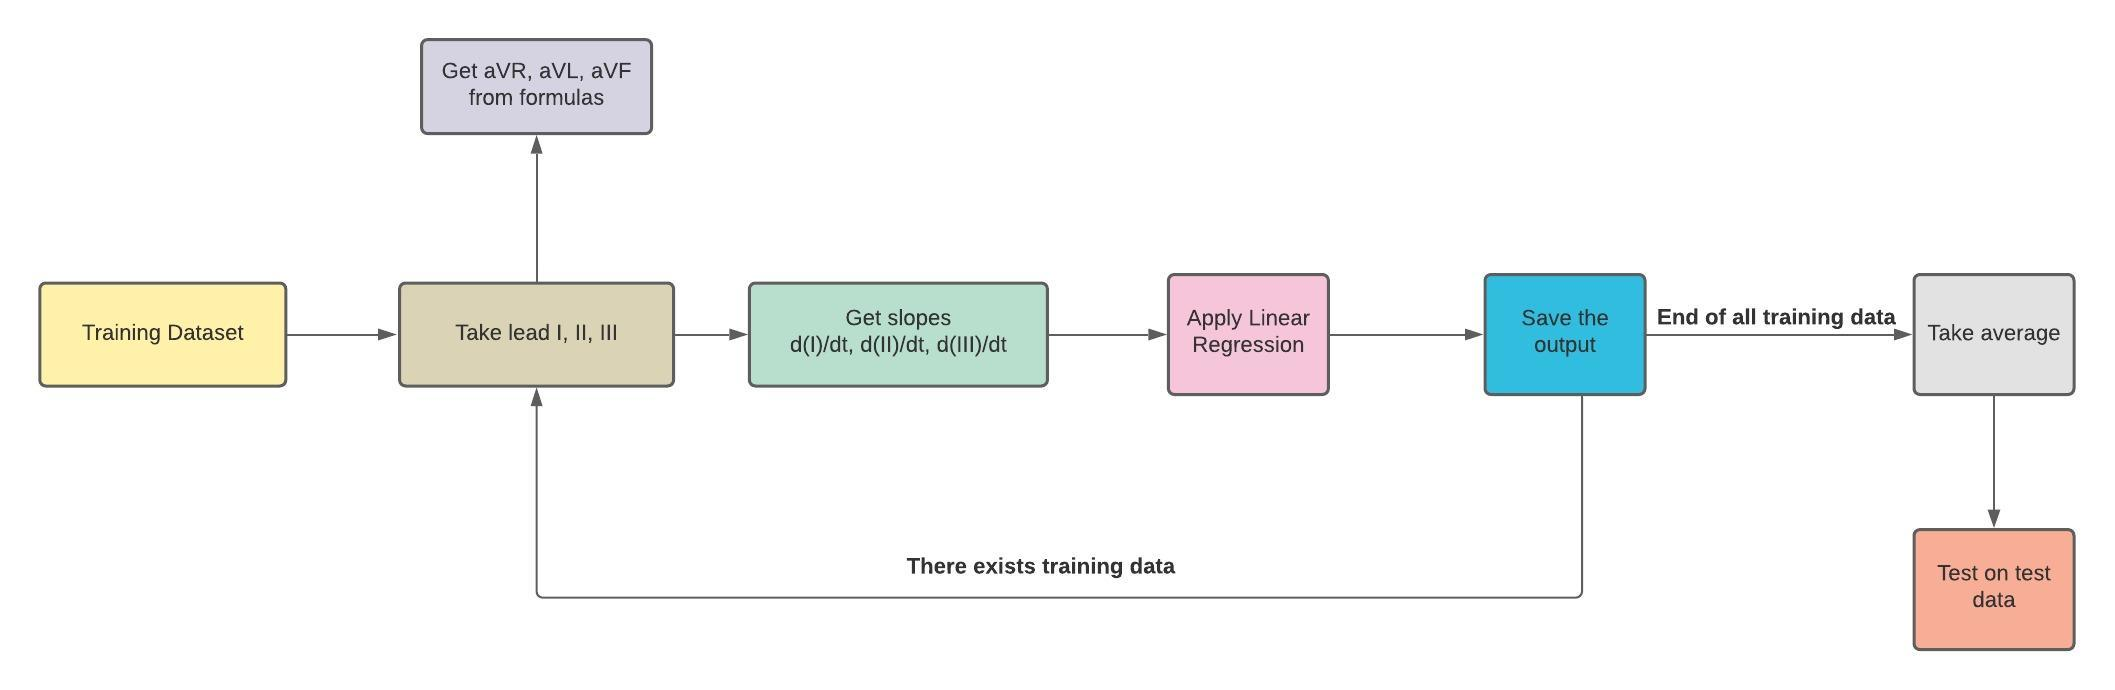
\includegraphics[width=\textwidth,height=\textheight,keepaspectratio]{save.jpeg} \begin{normalsize}
For each training set the fitting curve should be accurate enough so that the hypothesis parameter resulted can be used later for test cases. In one training case the resulting lead V1 and V2 fitting curves were as below\end{normalsize}\\
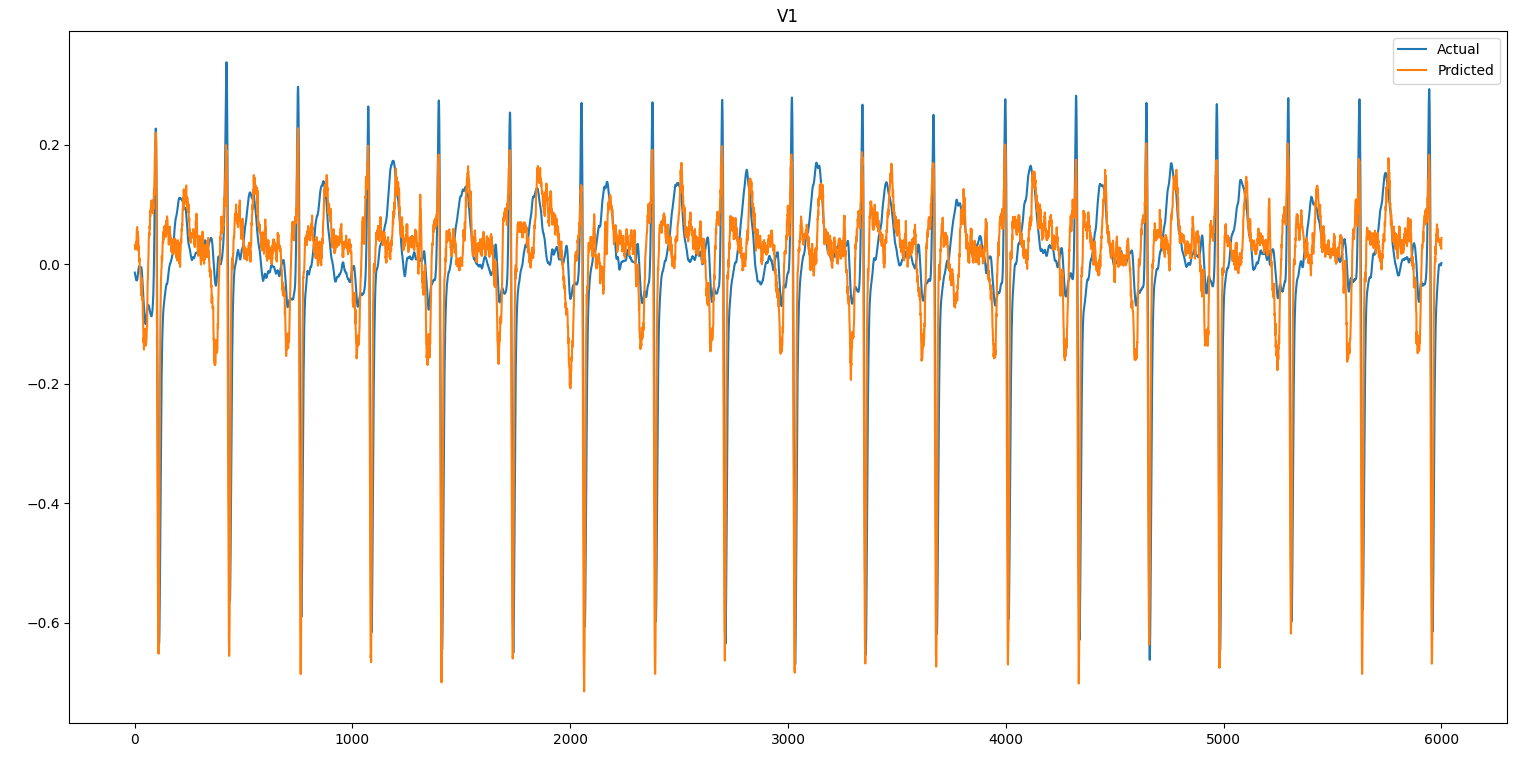
\includegraphics[width=\textwidth/2,height=\textheight,keepaspectratio]{Chapters/Figure_2_d.png}
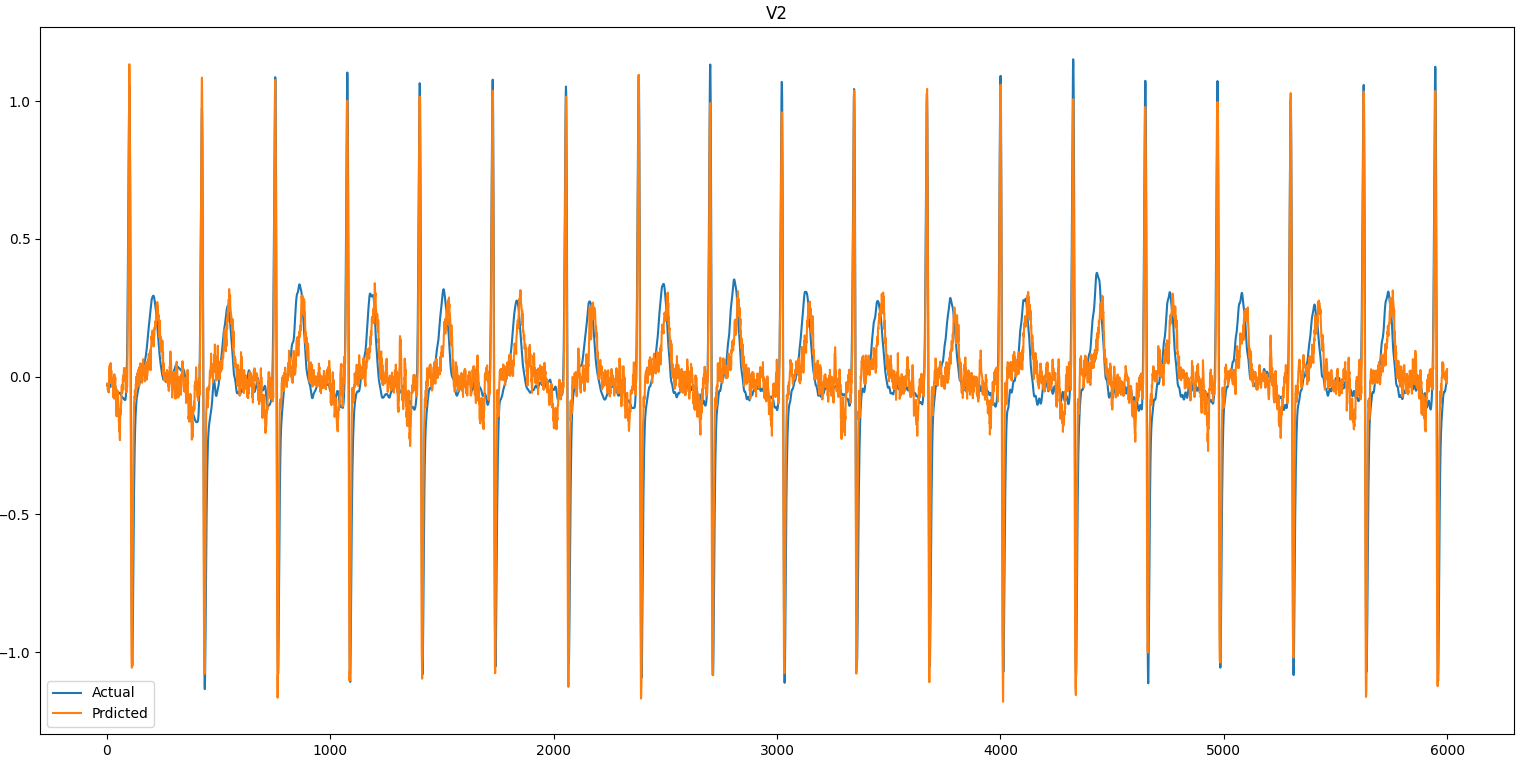
\includegraphics[width=\textwidth/2,height=\textheight,keepaspectratio]{Chapters/V2.png}\\Once we get the corresponding hypothesis parameters for each training instance it can be averaged together maybe by the weight inversely proportional by their errors in fitting to get an overall hypothesis parameter which can be tested on testing data. Also we should try to predict two out of 6 signal vectors in horizontal plane and then deduce other four from those two and compare the corresponding result with linear regression fitted approach. 

\section{Problems to be solved}
\begin{normalsize}
Linear regression was applied on a single training set to get hypothesis parameters but there is no guarantee that the weighted average may lead to acceptable model so as to apply in real world scenarios. \textbf{The first problem} is how should training instance be treated so as to handle the issue of over-fitting or under-fitting? \textbf{The second problem} is that the fitting curve got for each instance is time varied which needs to be processed so as to reduce error and remove excessive fluctuations.
At last, I need consider other prediction techniques like neural networks and SVM classifiers to see their accuracy rate and proceed further.In case of neural network approach the data will be cropped this might lead to data loss or might need to extrapolate this might give erroneous output. How to tackle such a situation?


\end{normalsize}


\bibliography{citations}
\bibliographystyle{rsc}
\end{document}

© 2021 GitHub, Inc.
Terms
Privacy
Security
Status
Docs
Contact GitHub
Pricing
API
Training
Blog
About
